\documentclass[../../index.tex]{subfiles}

\begin{document}
\chapter{Tau Decays into Hadrons}
The \(\tau\) lepton is an elementary particle with spin \(1/2\) and a mass of
\SI{1.77686}{\giga\eV} \cite{PDG2018}. It is the only lepton heavy enough to
decay into hadrons but also light enough for performing a low\-/energy
\textsc{qcd} analysis. Its inclusive hadronic\footnote{Meaning all decay
  channels with a hadron in its final state.} decay ratio is given by
\begin{equation}
  \label{eq:inclusiveRatio}
  R_\tau = \frac{\Gamma(\tau \to \nu_\tau + \text{hadrons})}{\Gamma(\tau \to \nu_\tau e^- \anti{\nu_e})}
\end{equation}
and sensible to the strong coupling, due to its rather large value, at the
\(m_\tau^2\) scale, of approximately \(0.33\). On the other hand
\(\alpha_s(m_\tau^2)\) is small enough to apply the \textsc{ope}. The
\textsc{np} \textsc{ope} contributions to the decay ratio are suppressed. The
dimension two contribution of the \textsc{ope} is proportional to the quark
masses and has only a tiny contribution for light quarks. The dimension four
contribution can be suppressed by applying weight functions, that do not have a
monomial in \(x\). E.g. the kinematic weight
\(\omega_\tau=(1-x)^2(1+2x)=1-3x^2+2x^3\) is not sensitive to \textsc{ope}
corrections of dimension four. The dimension six contribution of the
\textsc{ope} is proportional to \(1/(m_\tau^2)^3\) and further suppressed in the
\textsc{v+a} channel of the vector and axial\-/vector \(D=6\) contributions have
opposite signs and partly cancel themselves. Higher dimensional \textsc{ope}
contributions are suppressed by terms \(1/m_\tau^n\) with \(n \geq 8\). As a
result the perturbative contributions are dominant. They are known up to order
\(\mathcal{O}(\alpha_s^4)\) with a total contribution of \(20\%\) to \(R_\tau\)
\cite{Pich2016a}, which enables us to perform precise calculations of the
inclusive \(\tau\) decay ratio. Furthermore by extracting \(\alpha_s\) at low
energies at the scale of \(m_\tau^2\) we will achieve lower errors for the
strong coupling at higher energies as the errors run with the strong coupling
and get smaller with increasing energy.

The \(\tau\) decays permit one of the most precise determinations of the strong
coupling \(\alpha_s\). Building on the previously presented \textsc{qcdsr} we
will now elaborate the needed theory to extract \(\alpha_s\) from the process of
hadronic \(\tau\) decays.



\section{The Inclusive \(\tau\) Decay Ratio}
The theoretical expression of the inclusive hadronic \(\tau\) decay ratio
(\cref{eq:inclusiveRatio}) is given by
\begin{equation}
  \label{eq:hadronicTauDecayRatio}
  R_\tau(s) = 12 \pi S_{EW} \abs{V_{ud}}^2 \int_0^{m_\tau} \frac{\dif s}{m_\tau^2}
  \left( 1 - \frac{s}{m_\tau^2} \right)
  \left[ \left( 1 + 2 \frac{s}{m_\tau^2} \right) \Ima \Pi^{(1)}(s) + \Ima \Pi^{(0)}(s) \right],
\end{equation}
where \(S_{EW}\) is the electroweak correction, \(V_{ud}\) the corresponding
\define{ckm}{Cabibbo-Kobayashi-Maskawa} matrix element and $\Ima \Pi$ the
imaginary part of the two-point function. For brevity we will omit the
electroweak \(S_{EW}\) and \textsc{ckm} factors from now on.
\Cref{eq:hadronicTauDecayRatio} was first derived in \cite{Tsai1971}, using
current algebra, a more recent derivation making use of the \textit{optical
  theorem} can be taken from \cite{Schwab2002}. Notice that we used the standard
Lorentz decomposition into transversal (\(J=1\)) and longitudinal (\(J=0\))
components of \cref{eq:standardLorentzDecomposition} to display the hadronic
decay ratio (\cref{eq:hadronicTauDecayRatio}).

Applying Cauchy's theorem, as seen in \cref{eq:qcdSumRules}, to the
\cref{eq:hadronicTauDecayRatio} we can rewrite the line integral into a closed
contour integral
\begin{equation}
  \label{eq:rTauT+L}
  R_\tau = 6 \pi i \oint_{s=m_\tau} \frac{\dif s}{m_\tau^2}
  \left( 1 - \frac{s}{m_\tau^2} \right)
  \left[ \left( 1 + 2 \frac{s}{m_\tau^2} \right) \Pi^{(1)}(s) + \Pi^{(0)}(s) \right].
\end{equation}
It is convenient to work with a slightly different combination of transversal
and longitudinal components \(\Pi^{(1+0)}\), which has been defined in
\cref{eq:correlatorCombination} and is free of kinematic singularities. As a
result we can further rewrite the hadronic \(\tau\) decay ratio into
\begin{equation}
  \label{eq:tauDecayRatioTL}
  R_\tau = 6 \pi i \oint_{\abs{s}=m_\tau} \frac{\dif s}{m_\tau^2}
  \left( 1 - \frac{s}{m_\tau^2} \right)^2
  \left[ \left( 1 + 2 \frac{s}{m_\tau^2} \right) \Pi^{(1+0)}(s) - \left( \frac{2 s}{m_\tau^2} \right) \Pi^{(0)}(s) \right].
\end{equation}
In the case of \(\tau\) decays we only have to consider vector and axial-vector
contributions of decays into up, down and strange quarks.

With \cref{eq:tauDecayRatioTL} we have a suitable physical quantity that can be
theoretically calculated as experimentally measured. By using the \textsc{qcdsr}
we apply a closed contour integral of radius \(s_0\). As a result we
successfully avoid low energies at which the application of \textsc{pt} would
be questionable. For example if we would choose a radius with the size of the
\(\tau\) mass \(m_\tau \approx \SI{1.78}{\mega\eV}\) the strong coupling would
have a perturbatively safe value of \(\alpha_s(m_\tau^2)\approx 0.33\)
\cite{Pich2016}. Obviously we would benefit even more from a contour integral
over a bigger circumference, but \(\tau\) decays are kinematically limited by
their mass. Nevertheless there are promising \(e^+e^-\) annihilation data, which
yield valuable inclusive decay ratio values up to \SI{2}{\giga\eV}
\cite{Boito2018}\cite{Keshavarzi2018}.


\subsection{Renormalisation Group Invariance}
We have seen in \cref{sec:twoPointFunction}, that the two-point function is not
a physical quantity, as the dispersion relation (\cref{eq:dispersionRelation})
contains an unphysical polynom. Luckily for the vector correlator, appearing in
hadronic \(\tau\) decays, the polynom is just a constant. Consequently we can
take the derivative with respect to the momentum \(s\) to derive a physical
quantity from the two\-/point function:
\begin{tcolorbox}[ams equation,myformula]
  D(s) \equiv -s \od{}{s} \Pi(s).
\end{tcolorbox}
\(D(s)\) is called the \textit{Adler function} and fulfils, as all physical
quantities, the \textsc{rge} (\cref{eq:RGE}). The Adler function commonly has
separate definitions for the longitudinal plus transversal and the solely
longitudinal contributions:
\begin{equation}
  \label{eq:adlerFunction}
  D^{(1+0)}(s) \equiv -s \od{}{s} \Pi^{(1+0)}(s), \qquad D^{(0)}(s) \equiv \frac{s}{m_\tau^2} \od{}{s} (s \Pi^{(0)}(s)).
\end{equation}
The two\-/point functions in \cref{eq:tauDecayRatioTL} can now be replaced with
the help of partial integration
\begin{equation}
  \int_a^b u(x) V(x) \dif x = \left[ U(x) V(x) \right]_a^b - \int_a^b U(x) v(x) \dif x.
\end{equation}
We will perform two separate computations for the two cases \((1+0)\) and
\((0)\). Starting by the transversal plus longitudinal contribution we get:
\begin{equation}
  \begin{split}
    R_\tau^{(1)} &= \frac{6 \pi i}{m_\tau^2}
    \oint_{\abs{s}=m_\tau^2}\underbrace{ \left( 1 - \frac{s}{m_\tau^2} \right)^2
      \left( 1 + 2 \frac{s}{m_\tau^2} \right)
    }_{= u(x)} \underbrace{ \vphantom{\left( \frac{s}{m_\tau^2} \right)} \Pi^{(1+0)}(s)}_{=V(x)} \\
    &= \frac{6 \pi i}{m_\tau^2} \left\{ \left[ -\frac{m_\tau^2}{2} \left( 1 -
          \frac{s}{m_\tau^2} \right)^3 \left( 1 + \frac{s}{m_\tau^2} \right)
        \Pi^{(1+0)}(s) \right]_{\abs{s}=m_\tau^2} \right. \\
    &\quad+ \oint_{\abs{s}=m_\tau^2} \underbrace{-\frac{m_\tau^2}{2} \left( 1 -
        \frac{s}{m_\tau^2} \right)^3 \left( 1 + \frac{s}{m_\tau^2} \right)
    }_{=U(x)} \underbrace{\vphantom{\left( \frac{1}{m_\tau^2} \right)}\od{}{s}
      \Pi^{(1+0)}(s)}_{=v(x)}
    \left. \vphantom{\left[ \left( \frac{1}{m_\tau^2} \right) \right]} \right\} \\
    &= -3 \pi i \oint_{\abs{s}=m_\tau^2s} \frac{\dif s}{s} \left( 1 -
      \frac{s}{m_\tau^2} \right)^3 \left( 1 + \frac{s}{m_\tau^2} \right)
    \od{}{s} D^{(1+0)}(s)
  \end{split}
\end{equation}
where we fixed the integration constant to \(c=-\frac{m_\tau^2}{2}\) in the
second line and left the antiderivatives contained in the squared brackets
untouched. If we parametrise the integral appearing in the expression in the
squared brackets we can see that it vanishes:
\begin{equation}
  \left[ -\frac{m_\tau^2}{2} \left( 1 - e^{-i \phi} \right)^3 \left( 1 + e^{-i \phi} \right) \Pi^{(L+T)}(m_\tau^2 e^{-i \phi}) \right]_0^{2\pi} = 0,
\end{equation}
where \(s \to m_\tau^2 e^{-i \phi}\) and \((1 - e^{-i \cdot 0}) = (1 - e^{-i
  \cdot 2 \pi}) = 0\). Repeating the same calculation for the longitudinal part
yields
\begin{equation}
  \begin{split}
    R_\tau^{(0)} &= \oint_{\abs{s}=m_\tau^2} \dif s \left( 1 -
      \frac{s}{m_\tau^2} \right)^2
    \left( - \frac{2 s}{m_\tau^2} \right) \Pi^{(0)}(s) \\
    &= - 4 \pi i \oint \frac{\dif s}{s} \left( 1 - \frac{s}{m_\tau^2} \right)^3
    D^{(0)}(s).
  \end{split}
\end{equation}
Consequently combining the transversal with the longitudinal contribution
results in
\begin{equation}
  R_\tau = - \pi i \oint_{\abs{s}=m_\tau^2} \frac{\dif s}{s}
  \left( 1 - \frac{s}{m_\tau^2} \right)^3
  \left[ 3 \left( 1 + \frac{s}{m_\tau^2} D^{(1+0)}(s) + 4 D^{(0)}(s) \right) \right].
\end{equation}
It is convenient to define \(x=s/m_\tau^2\) such that we can rewrite the
inclusive ratio as
\begin{tcolorbox}[ams equation,myformula]
  \label{eq:rTauFinal}
  R_\tau = - \pi i \oint_{\abs{s}=m_\tau^2} \frac{\dif x}{x} (1 - x)^3 \left[ 3
    (1 + x) D^{(1+0)}(m_\tau^2 x) + 4 D^{(0)}(m_\tau^2 x) \right],
\end{tcolorbox}
which will be the final expression we will be using to express the inclusive
\(\tau\) decay ratio.



\section{Theoretical Computation of \(R_\tau\)}
The previously derived expression for the \(\tau\) decay ratio is at first
approximation equal to the number of colours \cite{Peskin1995}
\begin{equation}
  R_\tau \approx N_c.
\end{equation} 
If we take the perturbative \(\delta_{pt}\) and non\-/perturbative
\(\delta_{npt}\) contributions into account we can organise the vector and
axial\-/vector inclusive decay ratio as
\begin{equation}
  \label{eq:rTauContributions}
  R_{\tau,V/A}^\omega = \frac{N_c}{2} \left( 1 + \delta_{pt}^{\omega} + \delta_{npt}^{\omega} \right).
\end{equation}
Note that the factor \(1/2\) comes from the fact, that in the chiral limit the
vector and axial\-/vector contributions are equal. The dependence on the chosen
weight function \(\omega\) is reflected in the upper indices.

For the kinematic weight (\cref{eq:kinematicWeight}), which appears naturally in the \(tau\) decay ratio,
\begin{equation}
  \omega_\tau \equiv (1-x)^2(1+2x),
\end{equation}
we have a dominant perturbative contribution of \(\delta_{pt} \approx 20\%\) to
\(R_\tau\) \cite{Pich2013} and a minor, but not negligible, non\-/perturbative
contribution of \(\delta_{V+A}^{NP} \lesssim 1\% \) \cite{Jamin2013} for the
\(V+A\)\-/channel.

In the following we want to derive the theoretical expressions needed to
calculate both of the corrections to \cref{eq:rTauContributions} starting with
the perturbative one.


\subsection{The Perturbative Contribution}
The perturbative contribution \(\delta_{pt}\) to the inclusive \(\tau\) decay
ratio is corresponds to the first term of the \textsc{ope}. Currently the
perturbative expansion has been calculated to fourth order
\(\mathcal{O}(\alpha_s^4)\). Due to their role as dominant corrections their
uncertainties from unknown higher-order corrections dictate the final error of
the determination of the strong coupling \cite{Pich2016}.

We will treat the correlator in the chiral limit, in which the scalar and
pseudo\-/scalar contribution of the two\-/point function vanish and the axial
and vectorial contributions are equal. As a result we can focus ourselves on the
vector correlator \(\Pi_V(s)\), which can be expanded as a sum over different
orders of \(\alpha\) \cite{Beneke2008}:
\begin{equation}
  \label{eq:correlatorExpansion}
  \Pi_V^{(1+0)}(s) = - \frac{N_c}{12 \pi^2} \sum_{n=0}^\infty a_\mu^n \sum_{k=0}^{n+1} c_{n,k} L^{k} \quad \text{with} \quad L \equiv \ln \frac{-s}{\mu^2},
\end{equation}
where we defined \(a_\mu \equiv \alpha(\mu)/ \pi\). The coefficient \(c_{n,k}\)
up to two-loop order can be obtained by Feynman diagram calculations. With the
diagrams of \cref{fig:perturbativeContributionFeynmanDiagrams} we can calculate
the one\-/loop result of the correlator \cite{Jamin2006}
\begin{figure}
  \centering
  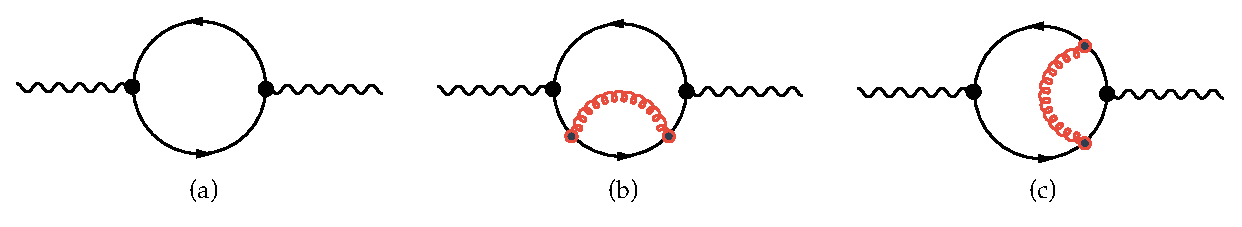
\includegraphics[width=\textwidth]{./images/correlatorLoopDiagrams.eps}
  \caption{Feynman loop diagrams to calculate the \(c_{n,k}\) coefficients of
    the expanded correlator \(\Pi_V^{(1+0)}\). The internal red lines represent
    gluons. Diagram a) represents the parton model and diagrams b) and c)
    represent higher order corrections.}
  \label{fig:perturbativeContributionFeynmanDiagrams}
\end{figure}
\begin{equation}
  \left. \Pi^B(q^2) \right\rvert^{1-loop} = \frac{N_c}{12\pi^2} \left( \frac{1}{\hat \epsilon} - \log\frac{(-q^2 - i0)}{\mu^2} + \frac{5}{3} + \mathcal{O}(\epsilon) \right),
\end{equation}
where \(\Pi^B_{\mu\nu}(q^2)\) is the bare two\-/point function\footnote{The term
  \(1/ \hat \epsilon\), which is of order zero in \(\alpha_s\), is not present
  in the Adler function or the imaginary part of the correlator.}. This result
can then be used to extract the first two coefficients of the correlator
expansion given in \cref{eq:correlatorExpansion}
\begin{equation}
  c_{0,0} = - \frac{5}{3} \qquad \text{and} \qquad c_{0,1} = 1.
\end{equation}

The second loop can also be calculated by diagram techniques resulting in
\cite{Boito2011}
\begin{equation}
  \left. \Pi_V^{(1+0)}(s) \right\rvert^{2-loop} = -\frac{N_c}{12\pi^2} a_\mu \log(\frac{-s}{\mu^2}) + \cdots
\end{equation}
yielding \(c_{1,1} = 1\).

Beginning from three loop diagrams the algebra becomes exhausting and one has to
use dedicated algorithms to compute the higher loops. The third loop
calculations have been done in the late seventies
\cite{Chetyrkin1979,Dine1979,Celmaster1979}. The four loop evaluation have been
completed a little more than ten years later
\cite{Gorishnii1990,Surguladze1990}. The highest loop published, that amounts to
\(\alpha_s^4\), was published in 2008 \cite{Baikov2008} almost 20 years later.

Fixing the number of colours to \(N_c=3\) the missing coefficients up to order
four in \(\alpha_s\) read:
\begin{equation}
  \label{eq:adlerCoefficients}
  \begin{split}
    c_{2,1} &= \frac{365}{24} - 11 \zeta_3 - \left( \frac{11}{12} - \frac{2}{3}\zeta_3 \right) N_f \\
    c_{3,1} &= \frac{87029}{288} - \frac{1103}{4} \zeta_3 + \frac{275}{6}\zeta_5 \\
    &- \left( \frac{7847}{216} - \frac{262}{9} \zeta_3 + \frac{25}{9} \zeta_5 \right) N_f + \left( \frac{151}{162} - \frac{19}{27}\zeta_3\right)N_f^2 \\
    c_{4,1} &= \frac{78631453}{20736} - \frac{1704247}{432}\zeta_3 +
    \frac{4185}{8}\zeta_3^2 + \frac{34165}{96}\zeta_5 - \frac{1995}{16}\zeta_7,
  \end{split}
\end{equation}
where used the flavor number \(N_f=3\) for the last line.

The 6-loop calculation has until today not been computed, but Beneke and Jamin
\cite{Beneke2008} used and educated guess to estimate the coefficient
\begin{equation}
  c_{5,1} \approx 283 \pm 283.
\end{equation}
We often see \(c_{5,1}\) applied to estimate the perturbative errors related to
missing higher order contributions.

In stating the coefficients \(c_{n,k}\) of the correlator expansion we have
restricted ourselves to \(k\) indices equal to one. This is due to the
\textsc{rge}, which relates coefficients with \(k\) different than one to
coefficients with \(k\) equal to one (\(c_{n,1}\)). Consequently the correlator
\(\Pi_V^{1+0}(s)\) needs to be a physical quantity, which we can be achieved
with the previously defined Adler function (\cref{eq:adlerFunction}). The
correct expression for the correlator expansion in \cref{eq:correlatorExpansion}
is then given by
\begin{tcolorbox}[ams equation,myformula]
  D_V^{(1+0)} = - s \od{\Pi_V^{(1+0)}(s)}{s} = \frac{N_c}{12 \pi^2}
  \sum_{n=0}^\infty a_\mu^n \sum_{k=1}^{n+1} k c_{n,k} L^{k-1},
\end{tcolorbox}
where we used \(\dif L^k/ \dif s=k\ln(-s/\mu^2)^{k-1}(-1/\mu^2)\). Applying the
\textsc{rge} (\cref{eq:RGE}) to the scale\-/invariant Adler function yields
\begin{equation}
  \label{eq:rgeAdler}
  -\mu \od{}{\mu} D_V^{(1+0)} = -\mu \od{}{\mu} \left( \pd{}{L} \dif L + \pd{}{a_s} \dif a_s \right) D_V^{(1+0)}
  = \left( 2\pd{}{L} + \beta \pd{}{a_s} \right) D_V^{(1+0)} = 0,
\end{equation}
where we made use of the \(\beta\)\-/function, which is defined in
\cref{eq:betaFunction}, and of the expression \(\dif L / \dif \mu = - 2/ \mu\).

The relation between the correlator expansion coefficients can then be taken by
calculating the Adler function for a desired order and plugging it into the
\textsc{rge}. For example the Adler function to the second order in \(\alpha_s\)
\begin{equation}
  \label{eq:adler2ndOrder}
  D(s) = \frac{N_c}{12 \pi^2} \left[ c_{01} + a_\mu(c_{11} + 2 c_{12} L) + a_\mu^2(c_{21} + 2 c_{22} L + 3 c_{23} L^2) \right],
\end{equation}
can be inserted into the \cref{eq:rgeAdler}
\begin{equation}
  4 a_\mu c_{12} + 2 a_\mu^2(2 c_{22} + 6 c_{23} L) + \beta_1 a_\mu^2(c_{11} + 2 c_{12}L) + \mathcal{O}(a_\mu^3) = 0
\end{equation}
to compare the coefficients order by order in \(\alpha_s\). At order
\(\alpha_\mu\) only the \(c_{12}\) term is present and has consequently to be
zero. For \(\mathcal{O}(a_\mu^2 L)\) solely \(c_{23}\) exists as \(c_{12}=0\)
and thus also has to vanish. Finally for \(\mathcal{O}(a)\) we can relate
\(c_{22}\) with \(c_{11}\) resulting in:
\begin{equation}
  c_{12} = 0, \quad c_{22} = \frac{\beta_1 c_{11}}{4} \quad \text{and} \quad c_{23} = 0.
\end{equation}
Implementing the newly obtained Adler coefficients we can write out the Adler
function to the first order:
\begin{equation}
  D(s) = \frac{N_c}{12 \pi^2} \left[ c_{01} + c_{11} a_\mu \left( c_{21} - \frac{1}{2} \beta_1 c_{11} L  \right) a_\mu^2 \right] + \mathcal{O}(a_\mu^3).
\end{equation}

We have used the \textsc{rge} to relate Adler function coefficients and thus
only need to know coefficients of type \(c_{n,1}\). Unfortunately, as we will
see in the following section, the \textsc{rge} gives us two different choices to
compute the perturbative contribution to the inclusive \(\tau\) decay ratio.

\subsubsection{Renormalisation group summation}
By making use of the \textsc{rge} we have to decide about the order of
mathematical operations we perform. As the all order perturbative contribution
\(\delta_{pt}}\) is independent on the scale \(\mu\) we are confronted with two
choices: \define{fopt}{fixed\-/order perturbation theory} and
\define{cipt}{contour\-/improved perturbation theory}. Each of them yields a
different result, which is the main source of error in extracting the strong
coupling from \(\tau\) decays.

Working in the chiral limit additionally permits us to neglect the longitudinal
contribution \(D^{(0)}\), in \cref{eq:rTauFinal} of the perturbative
contribution \(\delta_{pt}\) of \(R_\tau\) (\cref{eq:rTauContributions}). Thus
inserting the expansion of \(D_V^{(1+0)}\) into the hadronic tau decay width
\cref{eq:rTauFinal} yields
\begin{equation}
  \label{eq:rTauDelta0}
  \delta_{pt} = \sum_{n=1}^{\infty} a_\mu^n \sum_{k=1}^n k c_{n,k} \frac{1}{2 \pi i} \oint_{\abs{x}=1} \frac{\dif x}{x} (1-x)^3(1+x) \log \left( \frac{-m_\tau^2 x}{\mu^2} \right)^{k-1},
\end{equation}
where we kept in mind that the contributions from the vector and axial-vector
correlator are identical in the massless case.

To continue evaluating the perturbative part we can now either follow the
description of \textsc{fopt} or \textsc{cipt}. We will now present both.

In \textsc{fopt} we fix the scale at the tau mass (\(\mu^2=m_\tau^2\)), which
leaves us with the integration over the logarithm, as seen in
\begin{equation}
  \delta_{FOPT}^{(0)} = \sum_{n=1}^\infty a(m_\tau^2)^n \sum_{k=1}^n k c_{n,k} J_{k-1}
\end{equation}
where the contour integrals \(J_l\) are defined by
\begin{equation}
  J_l \equiv \frac{1}{2\pi i} \oint_{\abs{x}=1} \frac{\dif x}{x} (1-x)^3(1+x) \log^l(-x).
\end{equation}
The integrals \(J_l\) up to order \(\alpha_s^4\) are given by \cite{Beneke2008}:
\begin{equation}
  J_0 = 1, \quad J_1 = -\frac{19}{12} \quad J_2 = \frac{265}{72} - \frac{1}{3} \pi^2, \quad J_3 = - \frac{3355}{288} + \frac{19}{12}\pi^2.
\end{equation}
Using \textsc{fopt} the strong coupling \(a(\mu)\) is fixed at the tau mass
scale \(a(m_\tau^2)\) and can be taken out of the closed-contour integral. Thus
we solely have to integrate over the logarithms \(\log(x)\).

Using \textsc{cipt}, on the contrary, we can sum the logarithms by setting the
scale to \(\mu^2 = -m_\tau^2 x\) in \cref{eq:rTauDelta0}, resulting in:
\begin{equation}
  \delta^{(0)}_{CI} = \sum_{n=1}^\infty c_{n,1} J_n^a(m_\tau^2),
\end{equation}
where the contour integrals $J_l$ are defined by
\begin{equation}
  J_n^a(m_\tau^2) \equiv \frac{1}{2 \pi i} \oint_{\abs{x}=1} \frac{\dif x}{x} (1-x)^3(1+x) a^n(-m_\tau^2 x).
\end{equation}
Note that all logarithms vanish, except the ones with index \(k=1\):
\begin{equation}
  \log(1)^{k-1} =  \begin{cases} \mbox{1} & \mbox{if } k=1, \\ \mbox{0} & k\neq 1 \end{cases}
\end{equation}
which selects the Adler function coefficients \(c_{n,1}\). Handling the
logarithms left us with the integration of the strong coupling \(\alpha_s(-
m_\tau^2 x)\) over the closed-contour \(\oint_{\abs{x}=1}\), which now depends
on the integration variable \(x\).

In general we have to decide if we want to perform a contour integration with a
constant strong coupling parameter and variable logarithms (\textsc{fopt}) or
``constant logarithms'' and a running coupling (\textsc{cipt}). To emphasise the
differences in both approaches we can calculate the perturbative contribution
\(\delta^{(0)}\) to \(R_\tau\) for the two different prescriptions yielding
\cite{Beneke2008}
\begin{align}
  & \quad\qquad \alpha_s^2 \qquad \alpha_s^2 \qquad \alpha_s^3 \qquad \alpha_s^4 \quad\qquad \alpha_s^5 \nonumber\\
  \delta_{FOPT}^{(0)} &= 0.1082 + 0.0609 + 0.0334 + 0.0174 (+ 0.0088) = 0.2200 (0.2288) \\
  \delta_{CIPT}^{(0)} &= 0.1479 + 0.0297 + 0.0122 + 0.0086 (+ 0.0038) = 0.1984 (0.2021).
\end{align}
The series indicate, that \textsc{cipt} converges faster and that both series
approach a different value. \textsc{fopt} has larger contributions than
\textsc{cipt}, which leads to a smaller strong coupling if using \textsc{fopt}.
This discrepancy represents currently the biggest theoretical uncertainty for
extracting the strong coupling.

As today \textsc{fopt} or \textsc{cipt} are equally valid approaches to
calculate the perturbative contributions, even though it has been argumented by
Beneke et al. \cite{Beneke2008} to favour the former. Within this work we will
further elaborate the consistency of \textsc{fopt} and do not state our results
in \textsc{cipt}.

\subsection{The Non-Perturbative OPE Contributions}
The perturbative contribution to the sum rule is the dominant one, but
\textsc{np} have to be taken into account. The contribution of the \textsc{np}
part can be quoted as \cite{Jamin2013}
\begin{equation}
  \delta_{V+A,FOPT}^{NP} = -0.086(80), \qquad \delta_{V+A,CIPT}^{NP} = 0.0089(65)
\end{equation}
which is small, but not negligible. The \textsc{np} \textsc{ope} contributions
are commonly categorised by even, increasing dimensions. Contributions of
dimension larger than eight are normally neglected, due to the increasing
suppression by factors of \(1/m_\tau^{2\cdot D}\), where \(D\) stands for the
corresponding dimension.

The dimension two contributions are proportional to the quark masses and vanish
while working in the chiral limit. Consequently we will neglect them and start
by stating the \(D=4\) contributions.

\subsection{Dimension Four}
The next apparent \textsc{ope} contribution is of dimension four. Here we have
to take the terms with masses to the fourth power (\(m^4\)) into account, the
quark condensate multiplied by a mass (\(m \langle \anti{q} q \rangle\)) and the
gluon condensate (\(\langle GG \rangle\)). The resulting expression can be taken
from the appendix of \cite{Pich1999}, yielding:
\begin{equation}
  \left. D_{ij}^{(1+0)}(s) \right\rvert_{D=4} = \frac{1}{s^2} \sum_n \Omega^{(1+0)}(s/\mu^2)a^n,
\end{equation}
where
\begin{equation}
  \begin{split}
    \Omega_n^{(1+0)} (s/\mu^2) &\,=\, \frac{1}{6}\langle aGG \rangle p_n^{(1+0)}(s/\mu^2) + \sum_k m_k \langle \anti{q}_k q_k \rangle r_n^{(1+0)}(s/\mu^2) \\
    &\,+ 2\langle m_i \anti{q}_i q_i + m_j \anti{q}_j q_j \rangle q_n^{(1+0)} (s/\mu^2) \pm \frac{8}{3} \langle m_j \anti{q}_i q_i + m_i \anti{q}_j q_j \rangle t_n^{(1+0)} \\
    &\,- \frac{3}{\pi^2} (m_i^4 + m_j^4) h_n^{(1+0)} (s/\mu^2) \mp \frac{5}{\pi^2} m_i m_j (m_i^2 + m_j^2) k_n^{(1+0)}(s/\mu^2)\\
    &\,+ \frac{3}{\pi^2} m_i^2 m_j^2 g_n^{(1+0)}(s/\mu^2) + \sum_k m_k^4
    j_n^{(1+0)}(s/\mu^2) + 2 \sum_{k \neq l} m_k^2 m_l^2 u_n^{(1+0)}(s/\mu^2)
  \end{split}
\end{equation}
The perturbative expansion coefficients are known to second order
\(\mathcal{O}(a^2)\) for the condensate contributions,
\begin{equation}
  \begin{array}{lll}
    p_0^{(1+0)}=0, & p_1^{(1+0)}=1, & p_2^{(1+0)}=\frac{7}{6}, \\
    r_0^{(1+0)}=0, & r_1^{(1+0)}=0, & r_2^{(1+0)}=-\frac{5}{3}+\frac{8}{3}\zeta_3-\frac{2}{3}\log(s/\mu^2), \\
    q_0^{(1+0)}=1, & q_1^{(1+0)}=-1, & q_2^{(1+0)}=-\frac{131}{24}+\frac{9}{4}\log(s/\mu^2) \\
    t_0^{(1+0)}=0 & t_1^{(1+0)}=1, & t_2^{(1+0)}=\frac{17}{2}+\frac{9}{2}\log(s/\mu^2).
  \end{array}
\end{equation}
while the \(m^4\) terms have been only computed to first order
\(\mathcal{O}(a)\)
\begin{equation}
  \begin{array}{ll}
    h_0^{(1+0)}=1-1/2 \log(s/\mu^2), & h_1^{(1+0)}=\frac{25}{4}-2\zeta_3-\frac{25}{6}\log(s/\mu^2)-2 \log(s/\mu^2)^2, \\
    k_0^{(1+0)}=0, & k_1^{(1+0)}=1-\frac{2}{5}\log(s/\mu^2), \\
    g_0^{(1+0)}=1, & g_1^{(1+0)}=\frac{94}{9}-\frac{4}{3}\zeta_3-4 \log(s/\mu^2), \\
    j_0^{(1+0)}=0, & j_1^{(1+0)}=0, \\
    u_0^{(1+0)}=0, & u_1^{(1+0)}=0.
  \end{array}
\end{equation}

The above condensates all depend on the scale \(\mu^2\), but we can express them
in form of the scale\-/invariant gluon\-/ and quark\-/condensate
\cite{Spiridonov1988}, which are combinations of the minimally subtracted
operators
\begin{align}
  \beta_1 \langle a G^2 \rangle_I
  &\equiv \beta(s) \langle
    G_{(a)}^{\mu\nu}G_{\mu\nu}^{(a)} \rangle + 4 \gamma(a) \sum_{i=u,d} \langle
    m_i \anti{q}_i q_i \rangle \nonumber \\ 
  &- \frac{3}{4\pi^2} \sum_{i,j=u,d} m_i^2m_j^2
    \gamma_0^{ij}(a) \\
  \langle  m_i \anti{q}_j q_j \rangle
  &\equiv \langle \anti{q}_j q_j \rangle
    +\frac{3 m_i m_j^3}{7 \pi^2 a} \left\{ 1 - \frac{53}{24}a + \mathcal{O}(a^2) \right\},
\end{align}
where \(\gamma_0^{ij}(a) = -2 - 8/3 a\). During this work we will insert the
known invariant quark condensates (see \cref{table:constants}) as constants and
state our results for the invariant gluon condensate.


\subsection{Dimension Six and Eight}
Our application of dimension six contributions is founded in \cite{Braaten1991}
and has previously been calculated beyond leading order by \cite{Lanin1986}. The
operators appearing are the masses to the power six (\(m^6\)), the four\-/quark
condensates (\(\langle \anti q q \anti q q \rangle\)), the three-gluon
condensates (\(\langle g^3 G^3 \rangle\)) and lower dimensional condensates
multiplied by the corresponding masses, such that in total the mass dimension of
the operator will be six. The largest contributions comes from the 4\-/quark
operators. The three\-/gluon condensate does not contribute at leading order
\cite{Hubschmid1982} and is neglected. Operators proportional to the light quark
masses will also be neglected. The resulting contribution of dimension six
operators has been calculated in \cite{Lanin1986} and leads to a large amount of
operators, which until today cannot be accurately determined by phenomenology
methods. To reduce the number of operators we can make use of the
\define{vsa}{vacuum saturation approach}
\cite{Beneke2008,Braaten1991,Shifman1978} to express them in quark condensates
\(\langle q \anti{q} \rangle\). For Wilson coefficients of order \(\alpha_s\)
and applying the vacuum saturation we get a dimension six contributions of
\begin{equation}
  \left. D_{ij,V/A}^{1+0}(s) \right\vert_{D=6} = \frac{32\pi^2}{3} a(\mu) \frac{\langle \anti{q}_iq_i(\mu) \rangle\langle \anti{q}_jq_j \rangle}{s^3}
  - \frac{32}{7} \pi^2 a_\mu \frac{\langle \anti{q}_i q_i \rangle^2 \langle \anti{q}_j q_j \rangle^2}{s^3}.
\end{equation}
Unfortunately the scaling properties of the dimension six contribution,
resulting from the \textsc{vsa}, are inconsistent with the scaling properties of
the 4\-/quark operators \cite{Narison1983,Jamin1985} and terms of order
\(\alpha_s^2\) are usually ignored. In addition to the scaling problematic the
\textsc{vsa} is known to underestimate the dimension six contribution
\cite{Launer1983}.

In our work we take the simplest approach possible: Introducing an effective
dimension six coefficient \(\rho_{V/A}^{(6)}\) divided by the appropriate power
in s
\begin{equation}
  \left. D_{ij,V/A}^{(1+0)}(s) \right\rvert_{D=6} = 3 \frac{\rho_{V/A}^{(6)}}{s^3}.
\end{equation}

Here we also neglected the scale dependence of the dimension six operator, which
is determined by the anomalous dimension. We have calculated the
leading\-/order anomalous dimension matrices corresponding to the dimension\-/6
four\-/quark operators of flavour non\-/diagonal, as well as flavour diagonal,
mesonic vector and axial\-/vector currents in \cite{Boito2015}.

As for the dimension eight contribution the situation is not better than the
dimension six one we keep the simplest approach, leading to
\begin{equation}
  \left. D_{ij,V/A}^{(1+0)} \right\rvert_{D=8} = 4 \frac{\rho_{V/A}^{(8)}}{s^4}.
\end{equation}

The \textsc{np} contribution of dimension eight is the highest order that we are
going to implement. Higher orders will be neglected. Next to the \textsc{np}
treatment of the \textsc{ope} we have to discuss possible \textsc{dv}.



\section{Duality Violations}
As seen in \cref{sec:duality} we have to assume quark\-/hadron duality for the
\textsc{qcdsr} to work. Unfortunately duality is always to some extend broken
through so\-/called \textsc{dv}, which are well known
\cite{Cata2008,Cata2009}. Experimental data show an oscillating behaviour that
cannot be reproduced by the \textsc{ope}. Moreover in the large \(N_c\) limit it
can be shown that \textsc{dv} have an exponential decreasing, sinusoidal
appearance \cite{Cata2005}. Consequently for the cases with apparent \textsc{dv}
we have to somehow include the corrections coming from \textsc{dv} and adapt
\cref{eq:rTauContributions}, leading to
\begin{equation}
  R_{\tau,V/A}^\omega = \frac{N_c}{2}S_{EW} \abs{V_{ud}}^2 \left( 1 + \delta_{pt}^{\omega} + \delta_{npt}^{\omega} + \delta_{dv}^{\omega} \right),
\end{equation}
where we extracted \(\delta_{dv}\) from \(\delta_{npt}\), even though
\textsc{dv} are \textsc{np}. The \textsc{dv} correction has been modelled with
the following ansatz \cite{Cata2009}
\begin{equation}
  \label{eq:dvModel}
  \rho_{V/A}^{DV}(s) = e^{-(\delta_{V/A}+\gamma_{V/A}s)} \sin(\alpha_{V/A} + \beta_{V/A}s),
\end{equation}
which contains four parameters for the vector and another four parameters for
the axial\-/vector contribution. Note that for fitting the kinematic weight in
the \textsc{V}\-/channel, which is known to be sensible for \textsc{dv} at lower
energies \cite{Boito2011a}, we would have seven parameters instead of only
three. Making use of the model (\cref{eq:dvModel}) the \textsc{dv} then appear
as an additional term in the inclusive tau decay ratio
\begin{equation}
  R_{\tau,V/A} = - \pi i \oint_{\abs{s}=m_\tau^2} \frac{\dif x}{x} (1 - x)^3 \left[ 3
    (1 + x) D^{(1+0)}(m_\tau^2 x) + 4 D^{(0)}(m_\tau^2 x) \right] +  \mathcal{D}_{V/A}(m_\tau^2),
\end{equation}
where the \textsc{dv} contributions would be given as
\begin{equation}
  \mathcal{D}_\omega(m_\tau^2) = -12 \pi^2 \int_{m_\tau^2}^\infty \frac{\dif s}{m_\tau^2} \omega(s) \rho_{V/A}.
\end{equation}

\subsection{Pinched Weights to avoid DVs}
\label{sec:pinchedWeights}
The general \textsc{qcdsr} (\cref{eq:qcdSumRules}) contain a weight function
\(\omega\), which is not only used to suppress higher order dimensions, but also
\textsc{dv}. The weights that suppress \textsc{dv} are so\-/called pinched
weights of the form
\begin{equation}
  \omega(s) = \left(1-\frac{s}{m_\tau^2}\right)^k,
\end{equation}
where \(k\) is the degree of the pinched weight. The higher the degree of the
pinching, the lower the contribution of the critical region close to the real
axis (see. \cref{fig:monomialWeightGraphs}). Thus for higher pinchings we are
better protected from \textsc{dv} effects.
\begin{figure}
  \centering
  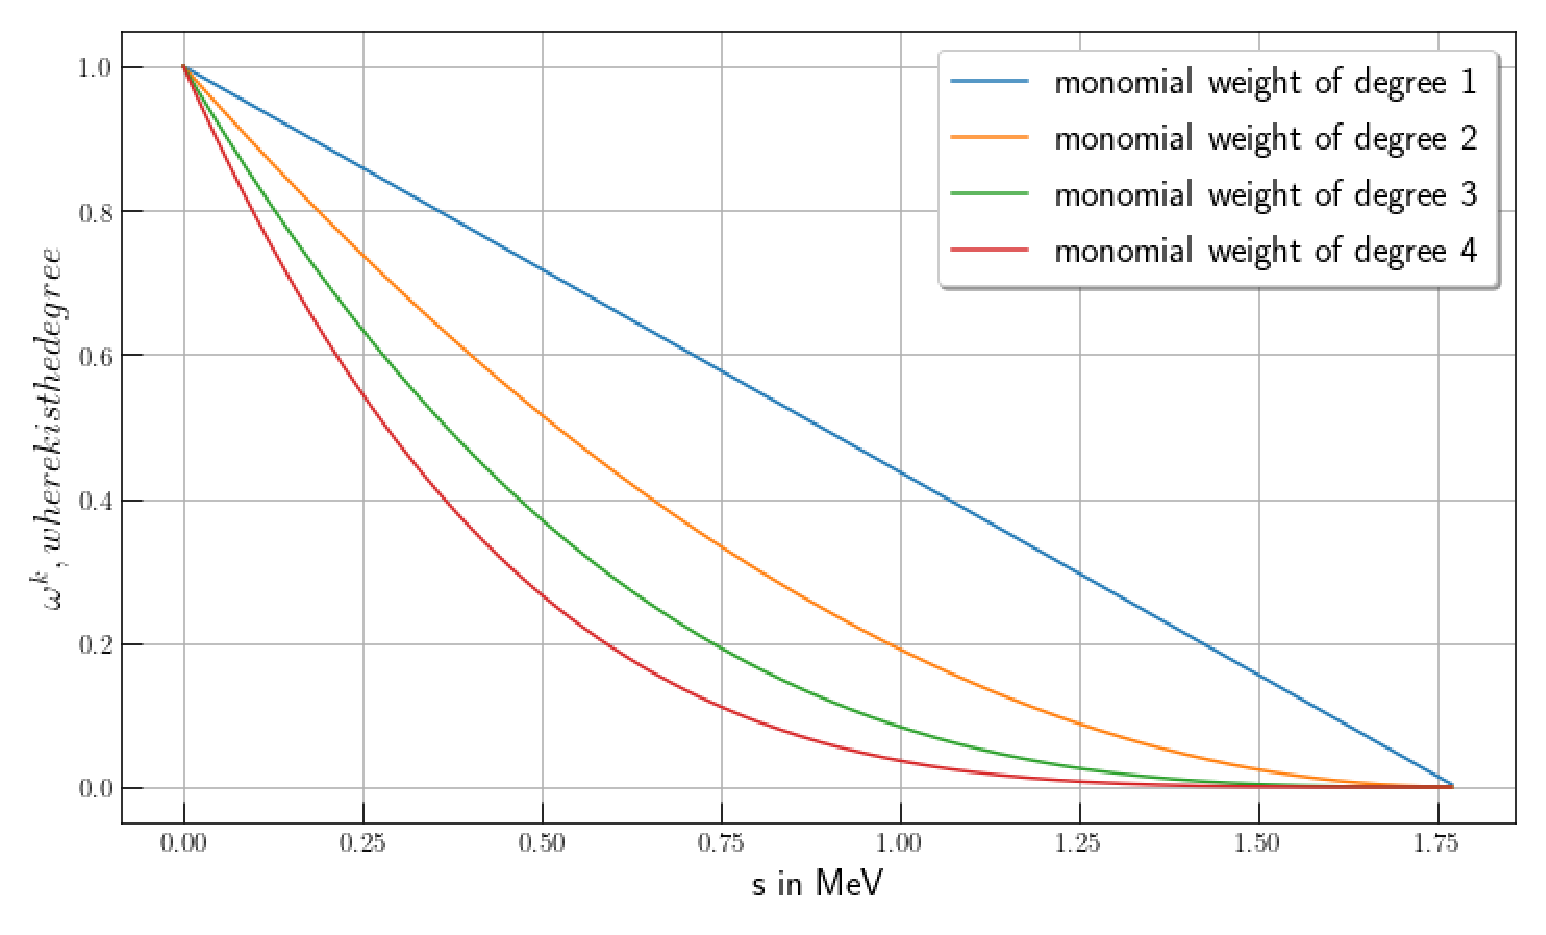
\includegraphics[width=\textwidth]{./images/monomialWeightGraphs.eps}
  \caption{Pinched weights \((1-s/m_\tau^2)^k\) for degrees \(1\) to \(4\). We
    can see that weights of higher pinching decrease faster, which comes in
    handy if we want to suppress duality violations.}
  \label{fig:monomialWeightGraphs}
\end{figure}
For the transversal component of the inclusive \(\tau\) decay ratio
(\cref{eq:rTauT+L}) a pinching of second degree appears quite naturally as the
kinematic weight (see \cref{eq:kinematicWeight}). In general it is said that a
double pinched weight is sufficient to neglect effects caused by \textsc{dv}. In
our analysis we show that double pinched weights indeed sufficiently suppress
\textsc{dv} and that even single pinched weights yield acceptable results.
Additionally to applying pinched weights we focus on combinations of vector and
axial\-/vector contributions, which as we will see, regarding the \textsc{aleph}
data have visibly suppressed \textsc{dv}.



\section{Borel Summation}
The Adler function of \cref{eq:adlerFunction} is given by a divergent asymptotic series.
We only know the needed Adler function coefficients \(c_{n,m}\) up to fifth
order. To get the best possible sum for such a series we can apply the
\define{bs}{Borel summation}. The \textsc{bs} is an long known summation method
for divergent series introduced by Émile Borel \cite{Emile1899}.

Regarding the sum
\begin{equation}
  A = \sum_{n=0}^{\infty} a_k
\end{equation}
we can introduce the faculty of \(n\), which can be rewritten in its integral
form
\begin{equation}
  A = \sum_{n=0}^\infty \frac{n!}{n!} a_k = \sum_{n=0}^{\infty} \frac{a_k}{n!} \int_0^\infty e^{-t} t^n \dif t.
\end{equation}
Interchanging the integral and the sum is referred to as the Borel integral
\begin{equation}
  A \equiv \int_0^\infty \dif t e^{-t} \sum_{n=0}^\infty \frac{a_k}{n!} t^n,
  \label{eq:borelSum}
\end{equation}
which contains the Borel transform
\begin{equation}
  B[A](t) = \sum_{n=0}^\infty \frac{a_k}{n!} t^n.
\end{equation}
The Borel integral is only valid for Borel transforms with no singularities
for real positive \(t\). In the cases of a valid Borel integral the
\textsc{bs} can now be used to get exact answers of divergent series, by first
applying the Borel transform and then integrating over it with the help of the
Borel integral.

In our case we want to calculate the \textsc{bs} of the Adler function given in
\cref{eq:adlerFunction} to argue if \textsc{fopt} or \textsc{cipt} gives the
better approximation to the \(\tau\) decay ratio. For convenience the Adler
function is redefined as
\begin{equation}
  \frac{12 \pi^2}{N_c} D_V^{1+0}(s) \equiv 1 + \widehat D(s) \equiv 1 + \sum_{n=0}^{\infty} r_n \alpha_s(\sqrt{(s)})^{n+1}.
\end{equation}
Then we apply the Borel transformation to \(\widetilde D\)
\begin{equation}
  B[\widehat D](t) \equiv \sum_{n=0}^{\infty} r_n \frac{t^n}{n!} \quad \text{with} \quad t \in \matbb{C}.
\end{equation}
As \(t\) is in general a complex number we can study the Borel transform in
the so\-/called Borel plane. The Borel plane for the Adler function is
visualised in \cref{fig:borelPlane}.
\begin{figure}
  \centering 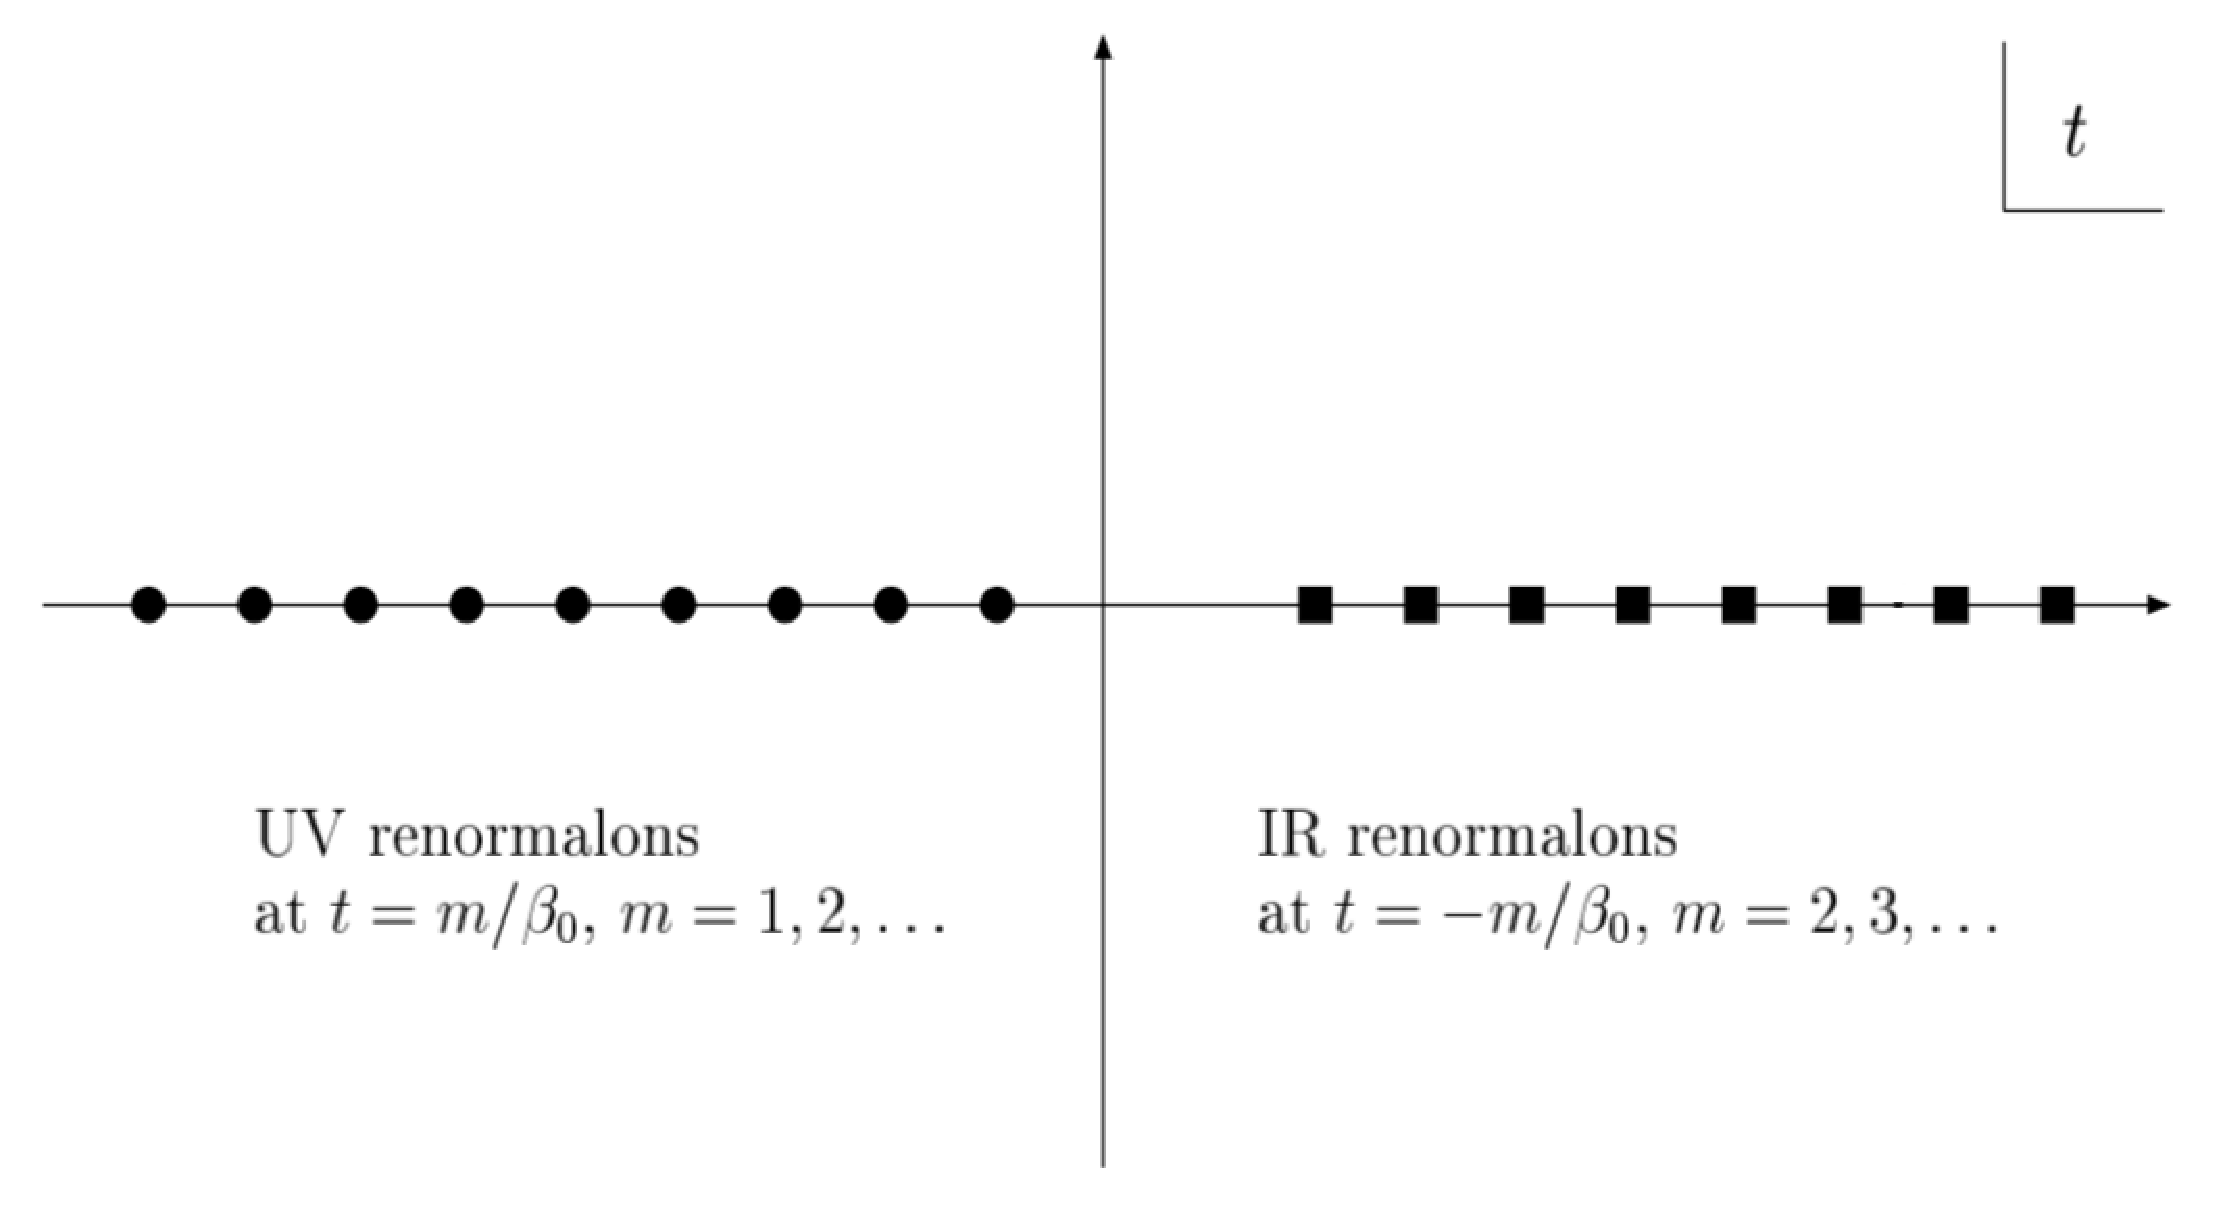
\includegraphics[width=\textwidth]{./images/borelPlane.eps}
  \caption{Singularities in the Borel plane of the Adler function, taken
    from\cite{Beneke1998}.}
  \label{fig:borelPlane}
\end{figure}
For real \(t\) the Borel transform of the Adler function has poles. Poles of
the Borel transform are referred to as renormalons \cite{Beneke1999,
  Zichichi1979}. We have to distinguish between \define{uv}{ultraviolet} and
\define{ir}{infrared} renormalons. \textsc{uv} renormalons are located at
\(t=m/\beta_0\) with positive integer \(m=1,2,\dots\) and \textsc{ir}
renormalons are located at \(t=-m\beta_0\) with positive integer
\(m=2,3,\dots\). Due to the poles of the positive real axis the Borel interal
\begin{equation}
  \widehat D(\alpha) \equiv \int_0^\infty \dif t e^{-t/\alpha} B[\widehat D](t)
\end{equation}
is not well defined. Consequently to have a valid Borel integral we have to
move the contour above or below the singularities.

The ansatz we use to express the Adler function in terms of the Borel sum was
introduced by Beneke et al. \cite{Beneke2008}. They have build a physical model
for the Adler function series
\begin{equation}
  \label{eq:borelModel}
  B[\widehat D](u) = B[\widehat D_1^{UV}](u) + B[\widehat D_2^{IR}](u) + B[\widehat D_3^{IR}](u) + d_0^{PO} + d_1^{PO}u,
\end{equation}
where \(B[\widehat D_p^{UV/IR}](u)\) are ansätze for the ultraviolet and
infrared appearing renormalon poles
\begin{align}
  B[\widehat D_p^{IR}](u)
  &\equiv \frac{d_p^{IR}}{(p-u)^{1+\tilde \gamma}}
    \left[  1 + \tilde b_1(p-u) + \tilde b_2(p-u)^2 + \dots \right] \\
  B[\widehat D_p^{UV}](u) &\equiv \frac{d_p^{UV}}{(p+u)^{1+\bar\gamma}}\left[1 + \bar b_1(p+u) + \bar b_2(p+u)^2 \right],
\end{align}
which have been defined in section five of \cite{Beneke2008}. As the large order
behaviour of the Adler function is governed by a sign\-/alternating \textsc{uv}
renormalon divergence and the lower\-/orders are not, only the leading
\textsc{uv} singularity has been included. Furthermore the intermediate orders
are governed by \textsc{ir} renormalons. Thus the first two (\(m=2\) and
\(m=3\)) have been included into the model. The five parameters \(d_1^{UV},
d_2^{IR}, d_3^{IR}, d_0^{PO}\) and \(d_1^{PO}\) have then to be matched to the
known perturbative expansion of the Adler function. They are found to be
\cite{Beneke2008}
\begin{equation}
  \begin{split}
    d_1^{UV} = -0.0156, \quad d_2^{IR} = 3.16, \quad d_3^{IR} = -13.5, \\
    d_0^{PO} = 0.781 \quad \text{and} \quad d_1^{PO} = 0.00766.
  \end{split}
\end{equation}

We will apply the Borel integral of this model to perform fits as an
alternative to \textsc{fopt} for the experimental data we are going to describe
in the upcoming section.



\section{Experiment}
The \(\tau\) decay data we use to perform our \textsc{qcd} analysis is from the
\textsc{aleph} experiment. The \textsc{aleph} experiment was located at the
\define{lep}{large\-/electron\-/positron} collider at \define{cern}{European
  Organisation for Nuclear Research} in Geneva. \textsc{lep} started producing
particles in 1989 and was replaced in the late 90s by the
\define{lhc}{large\-/hadron\-/collider}, which makes use of the same tunnel of
\SI{27}{\kilo\meter} circumference. The data produced within the experiment is
still maintained by former \textsc{aleph} group members led by M. Davier, which
have performed regular updates on the data-sets
\cite{Davier2013,Davier2008,Aleph2005}. The last update was motivated by Boito
et al. \cite{Boito2010}, who discovered irregularities in the covariances by
comparing data from a Monte Carlo generator with the \textsc{aleph}.

The measured spectral functions for the \textsc{aleph} data are defined in
\cite{Davier2007} and given for the transverse and longitudinal components
separately
\begin{equation}
  \begin{split}
    \rho^{(1)}_{V/A}(s) &= \frac{m_\tau^2}{12 \abs{V_{ud}}^2S_{EW}} \frac{\mathcal{B}(\tau^- \to V^-/A^- \nu_\tau)}{\mathcal{B}(\tau^- \to e^- \anti{\nu}_e \nu_\tau)} \\
    &\quad\times \frac{\dif N_{V/A}}{N_{V/A}\dif s} \left[ \left( 1 - \frac{s}{m_\tau^2} \right)^2 \left( 1 + \frac{2s}{m_\tau^2} \right) \right]^{-1} \\
    \rho^{(0)}_{A}(s) &= \frac{m_\tau^2}{12 \abs{V_{ud}}^2 S_{EW}}
    \frac{\mathcal{B}(\tau^- \to \pi^-(K^-) \nu_\tau)}{\mathcal{B}(\tau^- \to
      e^- \anti{\nu}_e \nu_\tau)} \times \frac{\dif N_A}{N_A \dif s} \left( 1 -
      \frac{s}{m_\tau^2} \right)^{-2}.
  \end{split}
\end{equation}

The data relies on a separation into vector and axial-vector channels. In the
case of the \(\pi\) this can be achieved via counting. The vector channel is
characterised by a negative G\-/parity, whereas the axial-vector channel has
positive G\-/parity. A single \(\pi\) carries negative G\-/parity, an even
number of \(\pi\) carries positive G\-/parity and an odd number of \(\pi\)
carries negative G\-/parity:
\begin{equation}
  n \times \pi = \begin{cases} \mbox{vector} & \mbox{if } n \text{ is even}, \\ \mbox{axial-vector} & \mbox{otherwise.} \end{cases}
\end{equation}
The separation into vector and axial\-/vector channel of mesons including
strange quarks, like \(K\anti{K}\) pairs, is more difficult, because these are
not in general eigenstates of G\-/parity and contribute to both \textsc{V} and
\textsc{A} channels.


The contributions to the spectral function for the vector, axial\-/vector and
V+A channel can be seen in \cref{fig:aleph}. The dominant modes in the vector
case are \cite{Davier2006} decays into two (\(\tau^- \to \pi^-\pi^0 \nu_\tau\))
or four (\(\tau^- \to \pi^- \pi^- \pi^+ \pi^0 \nu_\tau\)) pions. The first of
these is produced by an intermediate \(\rho(770)\) meson, which in contrary to
the pions carries angular momentum of one and is clearly visible as peak around
\(\SI{770}{\giga\eV}\) in \cref{fig:alephV}. The dominant modes in the
axial-vector case are decays into one (\(\tau^-\to \pi^-\nu_\tau\)) or three
(\(\tau^-\to \pi^- \pi^0 \pi^0 \nu_\tau\) and \(\tau^- \to \pi^- \pi^-
\pi^+\nu_\tau\)) pions. Here the three pion final states stem from the
\(a_1^-\)\-/meson, which can be seen as a peak in \cref{fig:alephA}.
\begin{figure}
  \centering
  \begin{subfigure}[b]{0.49\textwidth}
    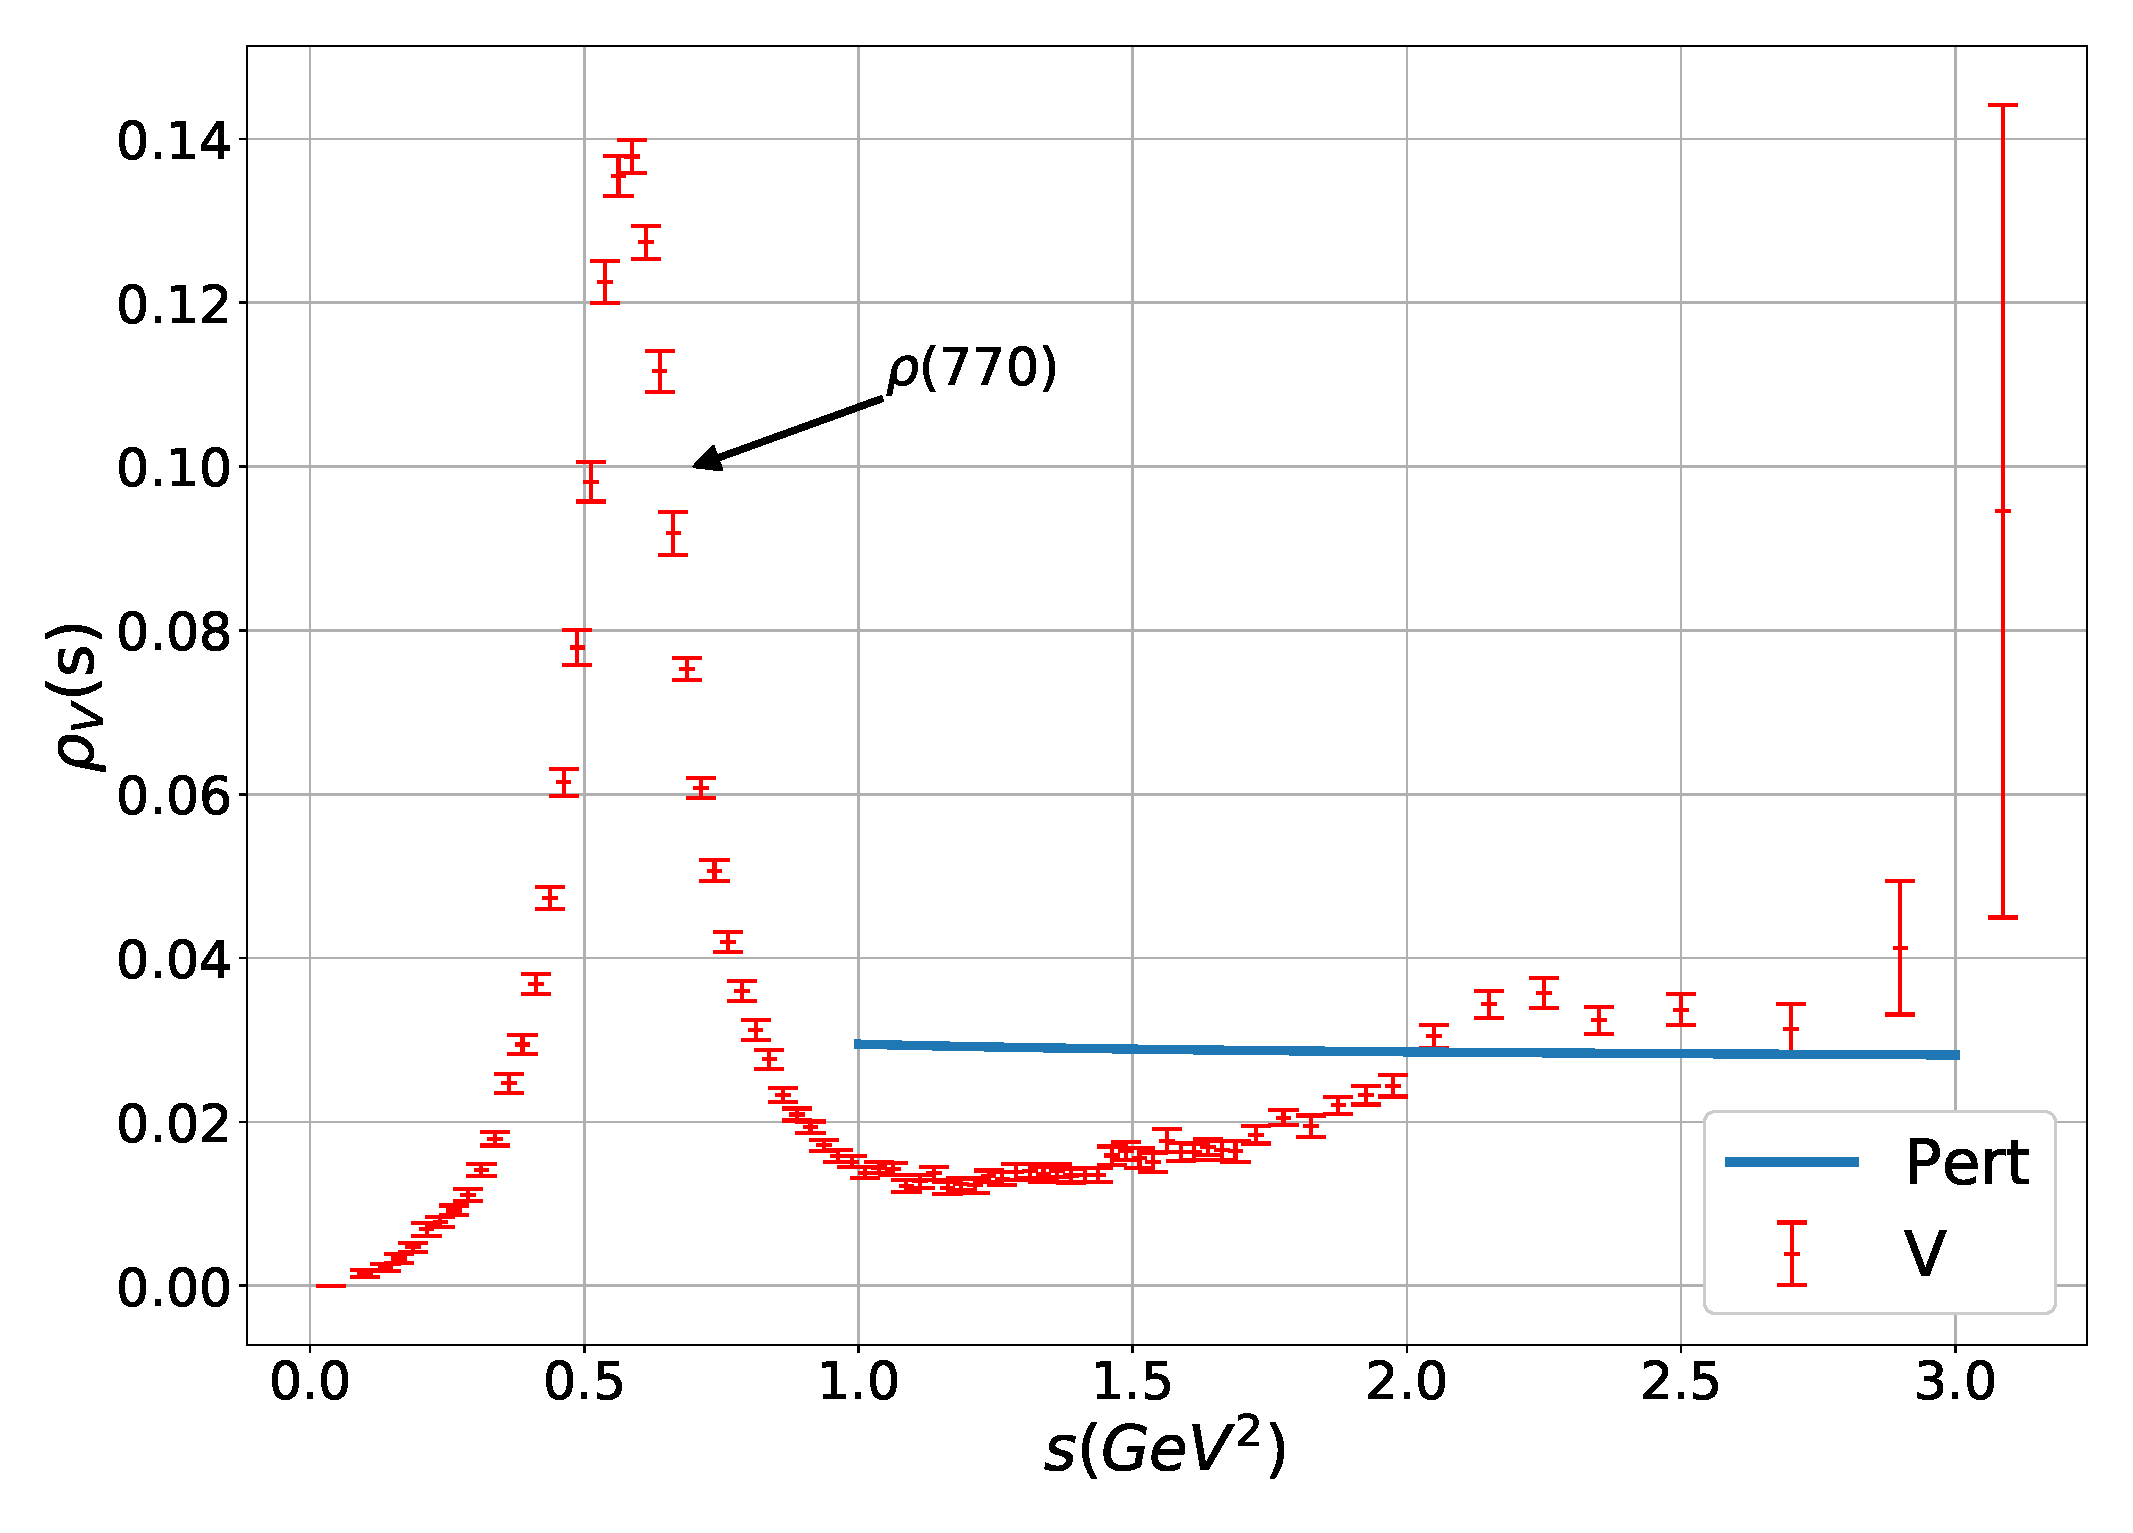
\includegraphics[width=\textwidth]{./images/specFuncAleph_V.eps}
    \caption{Vector}
    \label{fig:alephV}
  \end{subfigure}
  \begin{subfigure}[b]{0.49\textwidth}
    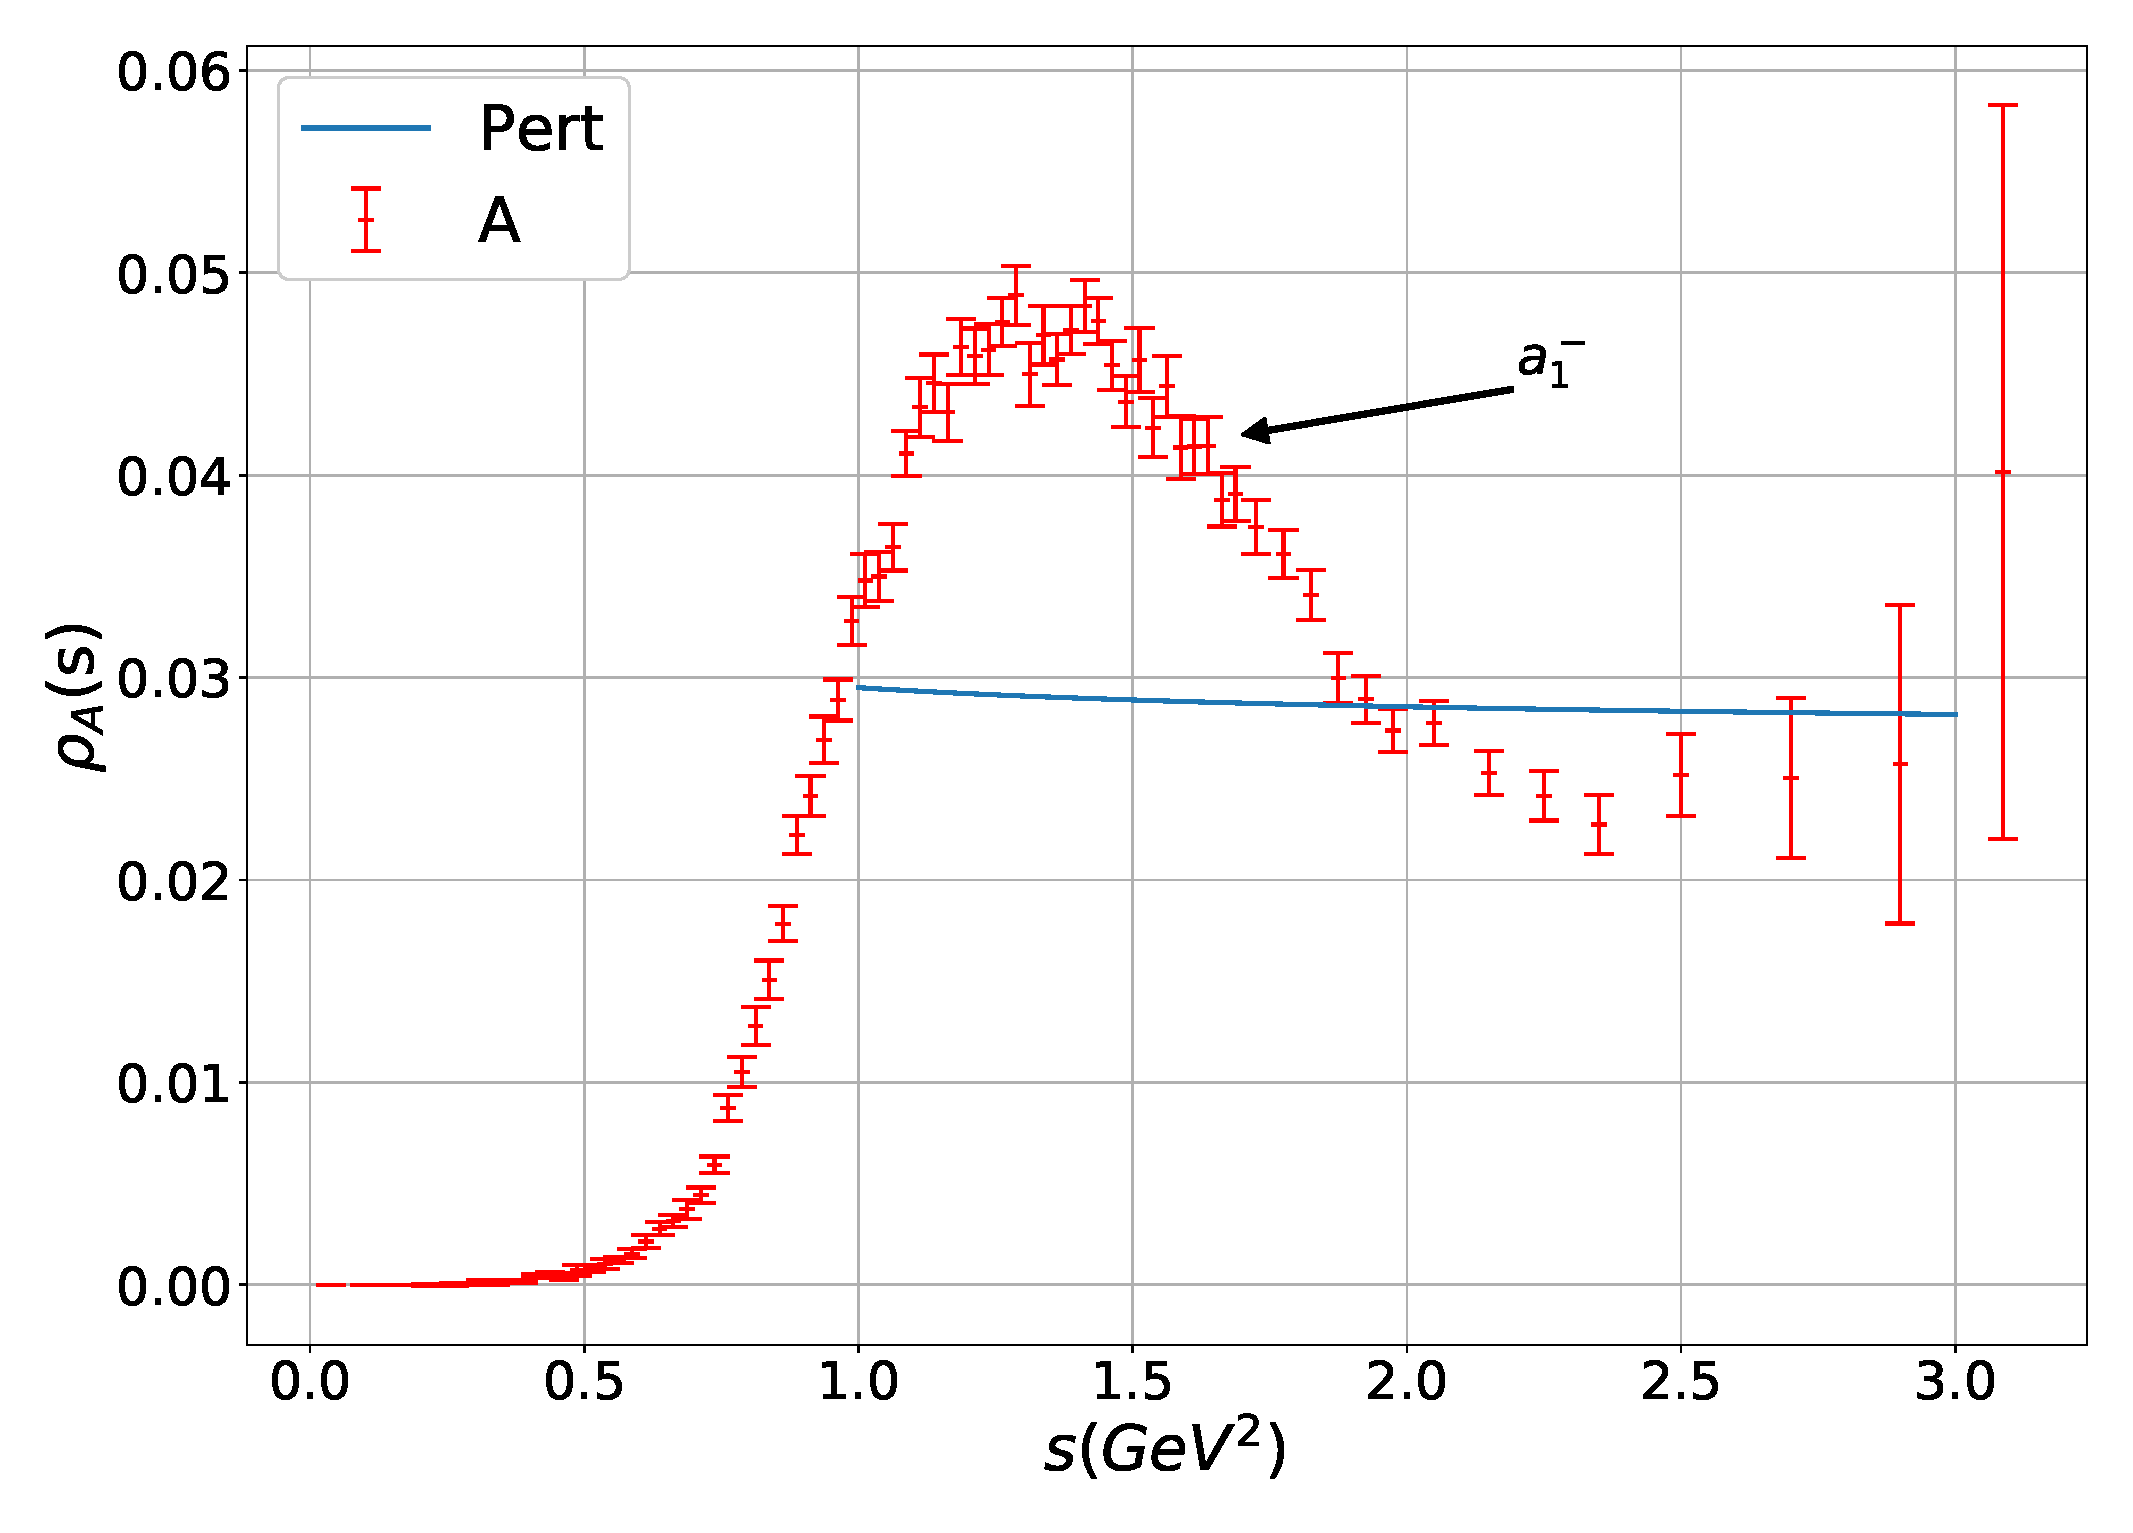
\includegraphics[width=\textwidth]{./images/specFuncAleph_A.eps}
    \caption{Axial-Vector}
    \label{fig:alephA}
  \end{subfigure}
  \begin{subfigure}[b]{\textwidth}
    \centering
    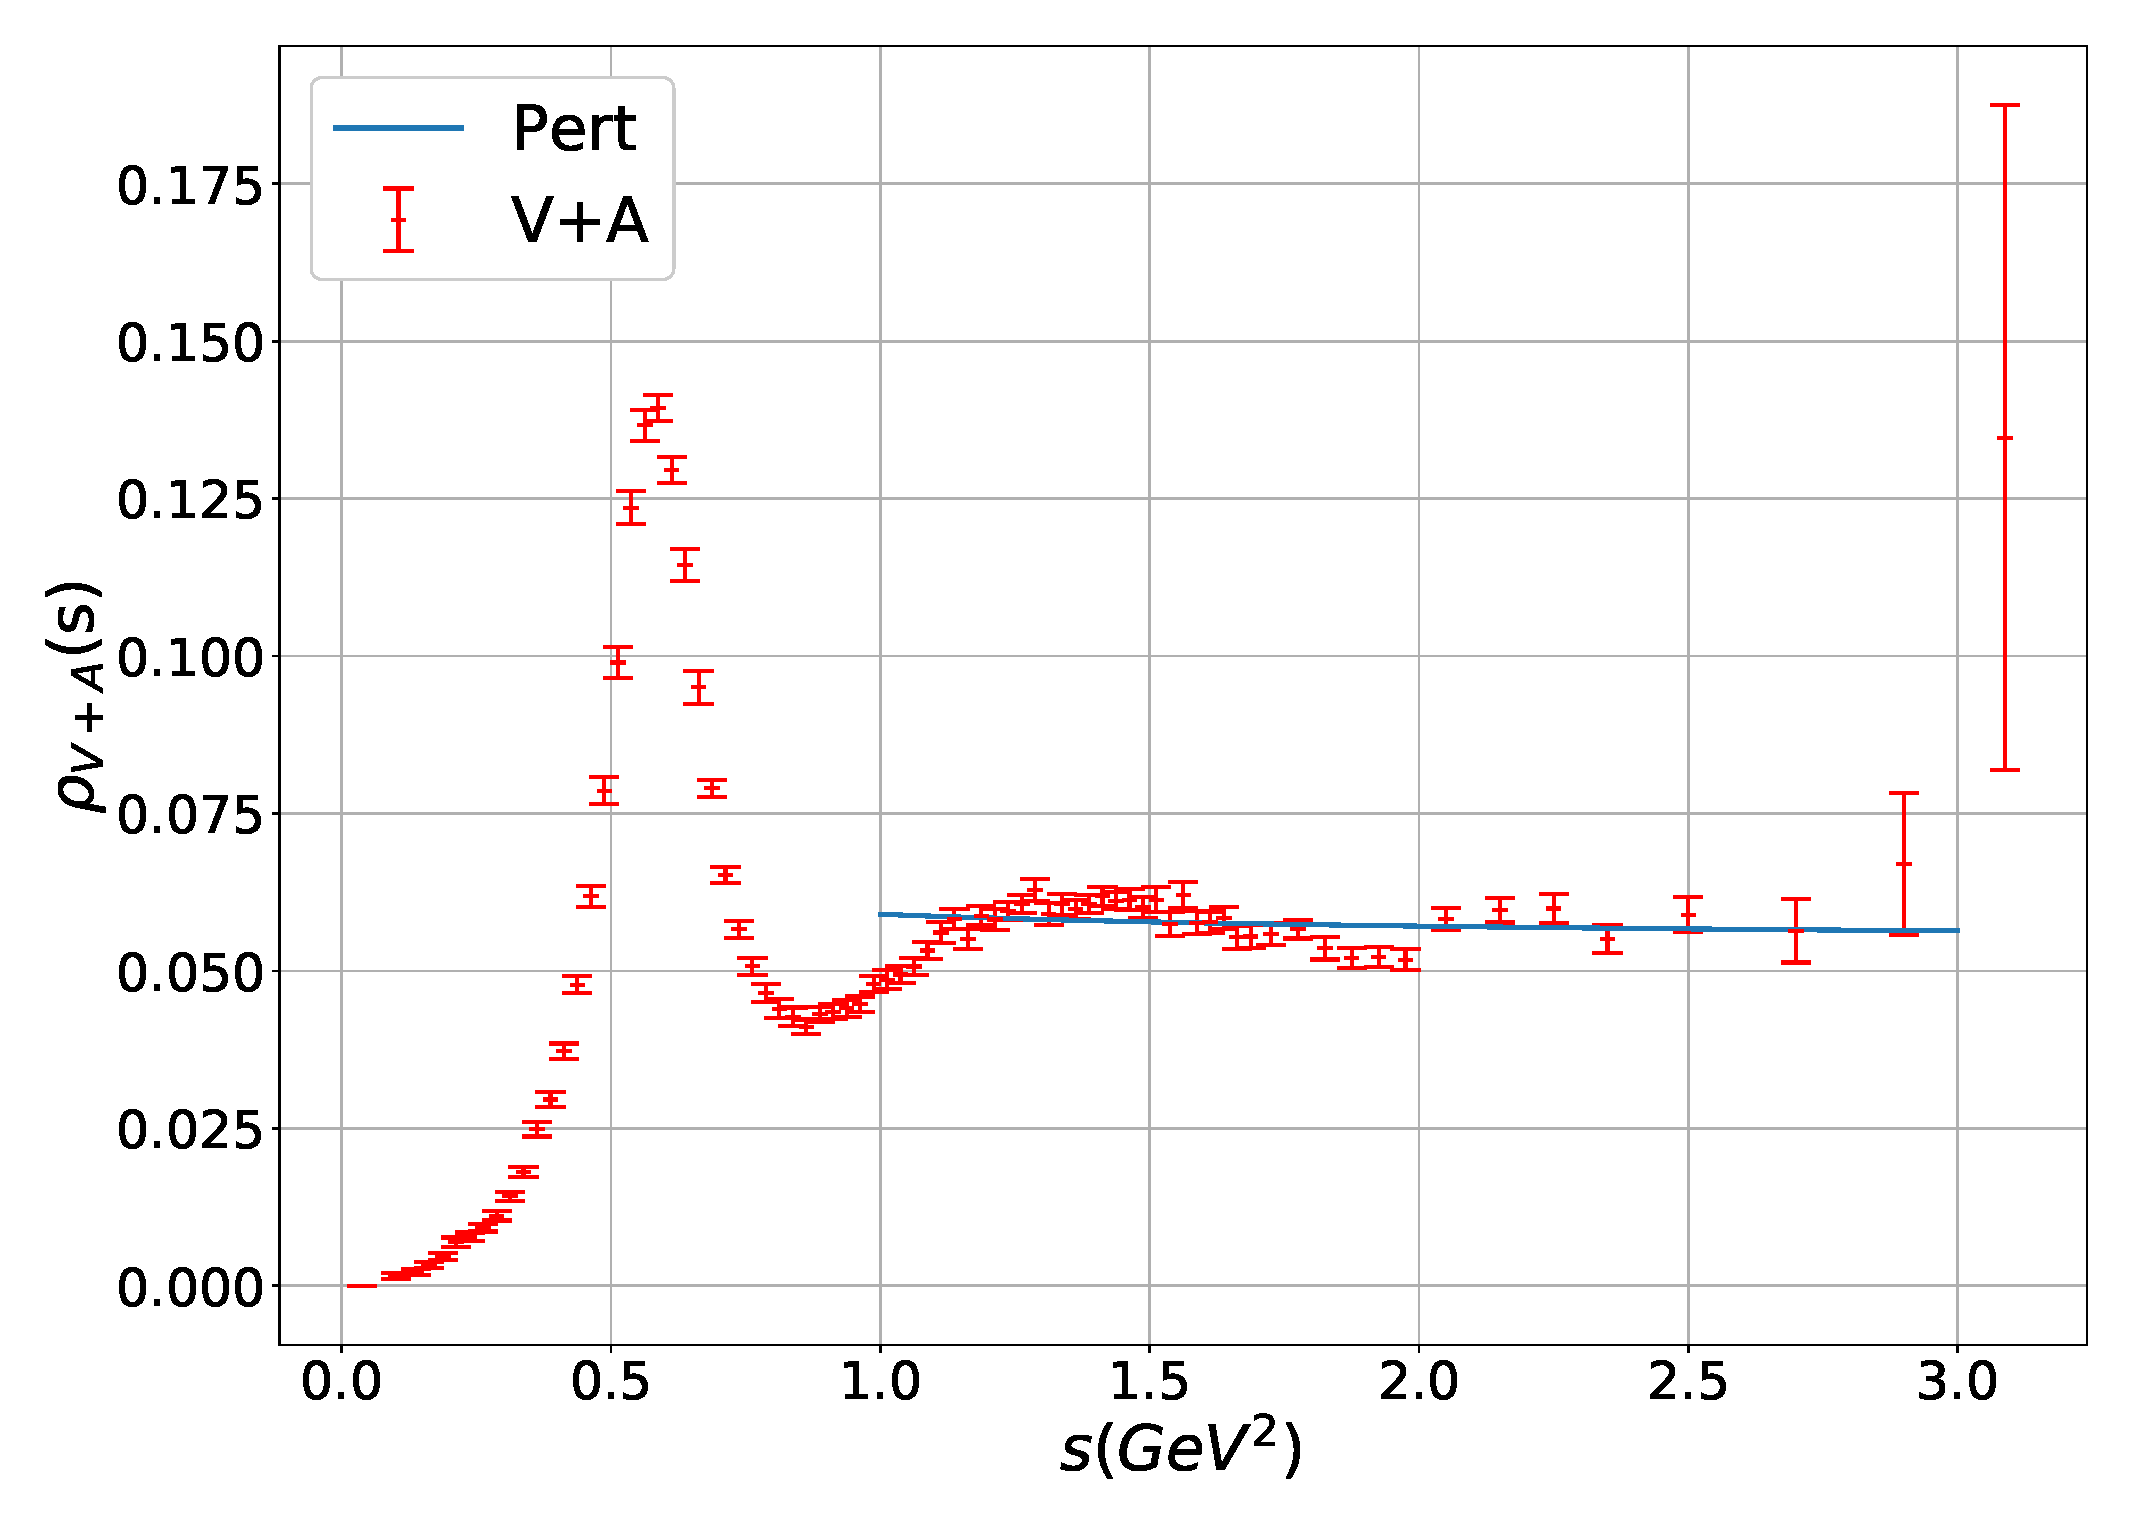
\includegraphics[width=\textwidth]{./images/specFuncAleph_VpA.eps}
    \caption{Vector plus Axial-Vector}
    \label{fig:alephVPlusA}
  \end{subfigure}
  \caption{Visualisation of the vector, axial\-/vector and V+A spectral function
    given by the \textsc{aleph} data \cite{Davier2013} in red with errors. We
    also plotted the \textsc{FOPT} theoretical calculation up to third order in
    \(\alpha_s\), for a fixed \(\alpha_s(\m_\tau)=0.329\) in blue. Note that the
    perturbative contribution can only limited represent the experimental data.
    It does not reproduce the sinusoidal form.}
  \label{fig:aleph}
\end{figure}

We furthermore added the perturbative contribution for a fixed
\(\alpha_s(m_\tau)=0.329\) using \textsc{fopt} in \cref{fig:alephVPlusA}. We can
see, that the perturbative contribution (the blue line) is an almost straight
line and cannot reproduce the oscillating behaviour, given by the \textsc{aleph}
data. This is especially the case for the \textsc{v} and \textsc{a} channel and
is seen as an indicator for \textsc{dv}. Even including \textsc{np}, higher
dimensions of the \textsc{ope} is not reproducing the wavy structure. In the
case of \textsc{v+a}, we have an higher agreement between our perturbative graph
and the data. In general we believe that \textsc{dv} are sufficiently suppressed
in the case of \textsc{v+a} and will argument in favour of this statement in the
following chapter. This is only the case for energies larger than
\SI{1.5}{\giga\eV}, as the \(\rho\) resonance of the \textsc{v} channel is
impossible to be represented by perturbative tools. For lower energies
\textsc{dv} become too important to be neglected.

\subsection{Total decay ratio from experimental data}
The data has been last revised in 2014 \cite{Davier2013} and is publicly
available \cite{AlephData}. It consists of the mass squared bin center
(\textit{sbin}), the bin size (\textit{dsbin}), the normalised invariant mass
squared distribution (\textit{sfm2}), the total errors (\textit{derr}) and their
correlations (\textit{corerr}). To make the data comparable to our theoretical
calculations we have to give the normalised invariant mass squared distribution
(\textit{sfm2}) in form of the total decay ratio \(R_\tau\). The data is given
as the normalised invariant mass squared distribution \((\dif N_i/\dif s)/N_i\)
scaled by a factor \(100\) and further normalised to the corresponding branching
ratio \(i\in\{\text{V,A,V+A}\}\). Thus we can connect the branching ratio of the
\(i\)\-/channel to \textit{sfm2} as follows
\begin{equation}
  \mathcal{B}_{V/A} \equiv \int_0^{s_\tau} \dif s \frac{\sfm2_{V/A}(s)}{100}
  \equiv \int_0^{s_\tau} \dif s \mathcal{B}_{V/A}
  \left( \frac{\dif N_{V/A}}{N_{V/A}\dif s} \right),
\end{equation}
where we used \(s_\tau \equiv m_\tau^2\). The total decay ratio \(R_\tau\) is
defined as the decay width of \(\tau\) decaying into hadrons over \(\tau\)
decaying into electrons. It and can be expressed via the corresponding branching
ratios, which can be connected to the invariant mass squared distribution
\(\sfm2\)
\begin{equation}
  R_{\tau, V/A} = \frac{\mathcal{B}_{V/A}}{\mathcal{B}_e}
  = \int_0^{s_\tau} \dif s \frac{\sfm2_{V/A}(s)}{100 \mathcal{B}_e}.
\end{equation}
Theoretically the decay ratio is given in \cref{eq:inclusiveRatio}. If we
neglect the longitudinal contribution \(\Ima \Pi^{(0)}(s)\) and remember the
definition of the spectral function (\cref{eq:spectralFunction}) and the
kinematic weight (\cref{eq:kinematicWeight}), we can write the decay ratio as
\begin{equation}
  R_{\tau, i} = \int_0^{s_\tau} \frac{\dif s}{s_\tau} \omega_\tau(s) \rho(s)
\end{equation}
and thus relate the spectral function to the experimental data
\begin{equation}
  \rho(s) = \frac{s_\tau}{12 \pi^2 100 \mathcal{B}_e} \frac{\sfm2}{\omega_\tau}.
\end{equation}
To fit the experimental data we define a so\-/called \textit{spectral function
  moment} (or \textit{moment})
\begin{equation}
  I_{i}^{exp, \omega} \equiv \int_0^{s_0} \frac{\dif s}{s_0} \omega\left( \frac{s}{s_0} \right) \rho(s),
\end{equation}
which will be used in our \(\chi^2\) fits, explained in the upcoming section.
The data is given for discrete bins so we have to express the integral of the
spectral function moment as sum over those bins. The final expression we use to
fit parameters to the experimental data is then given by
\begin{tcolorbox}[ams equation,myformula]
  I_{exp, V/A}^{\omega}(s_0) = \frac{s_\tau}{100 \mathcal{B}_e s_0}
  \sum_{i=1}^{N(s_0)} \frac{\omega\left( \frac{s_i}{s_0}
    \right)}{\omega_\tau\left( \frac{s_i}{s_\tau}\right)} \sfm2_{V/A}(s_i).
\end{tcolorbox}

\section{The Method of Least Squares}
We apply \define{ls}{method of least squares} to fit the parameters
\(\vec\alpha\) from the experimental data. Our \(\chi^2\)\-/function can be
expressed as
\begin{equation}
  \label{eq:ls}
  \chi^2 = \left( I_i^{exp} - I_i^{th}(\vec\alpha) \right) C^{exp}_{ij}^{-1} \left( I_j^{exp} - I_j^{th}(\vec\alpha) \right),
\end{equation}
where \(I^{exp}\)/\(I^{th}\) is a vector of experimental moments/ theoretical
moments with the same weight, but different energy cutoffs \(s_0\), labelled by
the index \(i\). In addition \(C^{exp}\) is the covariance matrix describing the
correlation of the different experimental moments
\(C_{ij}^{exp}=cov[I_i^{exp}I_j^{exp}]\), which can be computed by the given
correlation matrix of the \textsc{aleph} data.

In general we aim to minimise the value of \(\chi^2\), which will fix the
parameter vector \(\vec\alpha\). The properties of the \(\chi^2\)\-/function are
well known and the best fits are characterised through \(\chi^2/dof\approx 1\),
where the \textsc{dof} of the fit can be calculated through
\begin{equation}
  \text{#\textsc{dof}} = \text{#experimental moments} - \text{#parameters}.
\end{equation}
E.g. if we want to fit \(\alpha_s\) and the dimension four Wilson coefficient
\(C_4\) we get \(7-2=5\) \textsc{dof}.

For our purposes we use the numerical minimisation computer program
\textsc{minuit}, which was originally written in \textsc{fortran} by Fred James
in the 1970 \cite{James1975}. Today in its second version the program has been
ported to C++ by the \textsc{root} \cite{Brun1997} project at \textsc{cern}.

The parameter vector \(\vec\alpha\) includes the strong coupling \(\alpha_s\),
but also the included \textsc{ope} Wilson coefficient. Consequently we should
have at least as many, if not more moments as parameters we want to fit. As the
moments for different \(s_0\) are highly correlated we are limited to fit a set
of only a few parameters.

It is also possible to increase the number of moments used by applying multiple
weights \(\omega\). Unfortunately using different weights leads to highly
correlated moments, which cause numerical complications by inverting the
covariance matrix in \cref{eq:ls}. To handle the high correlations we have to
redefine our fit quality.


\subsection{Block Diagonal ``Fit\-/Quality''}
For fits including multiple weights, which we do not perform in this work, we
can redefine \textsc{ls} \cite{Boito2014} to
\begin{tcolorbox}[ams equation,myformula]
  Q^2 = \sum_{\omega} \sum_{s_0^i,s_0^j} \left(I_{\omega}^{exp}(s_0^i) -
    I_{\omega}^{th}(s_0^i,\vec\alpha)\right) \widetilde{C}_{ij,\omega}^{-1}
  \left(I_{\omega}^{exp}(s_0^j) - I_{\omega}^{th}(s_0^j,\vec\alpha)\right),
\end{tcolorbox}
where the covariance matrix \(\widetilde{C}\) is now a diagonal of the
experimental covariance matrices \(C_{\omega}^{exp}\) for each weight
\begin{equation}
  \widetilde{C} = \begin{pmatrix}
    C_{\omega=1}^{exp} & 0           & \dots  & 0      \\
    0           & C_{\omega=2}^{exp} & \ddots & \vdots \\
    \vdots      & \ddots      & \ddots & 0      \\
    0           & \dots       & 0      & C_{\omega=n}^{exp}
  \end{pmatrix}.
\end{equation}
As a result we are still able to invert the newly defined covariance matrix
\(\widetilde{C}\), but minimisation routines like \textsc{CERN} \textsc{minuit}
are not able to calculate the proper errors for the parameters we want to
extract. We have to perform our own error propagation to obtain meaningful
errors for the parameters. The error propagation has been derived in
\cite{Boito2011a,Boito2011} and is given as
\begin{equation}
  \langle \delta \alpha_k \alpha_l \rangle = A_{km}^{-1}A_{ln}^{-1}
  \pd{I_i^{th}(\vec\alpha)}{\alpha_m} \pd{I_r^{th}(\vec \alpha)}{\alpha_n}
  \widetilde{C}_{ij}^{-1} \widetilde{C}_{ij}^{-1} \langle \delta I_k^{exp} \delta I_l^{exp} \rangle,
\end{equation}
where
\begin{equation}
  A_{kl} = \pd{I^{th}(\vec\alpha)}{\alpha_k} \widetile{C}_{ij}^{-1} \frac{I^{th}_j(\vec\alpha)}{\alpha_l}.
\end{equation}
\end{document}
% LocalWords:  adlerFunction rTauContributions adlerSndOrder betaFunction rTauT
% LocalWords:  correlatorExpansion correlatorLoopDiagrams antiderivatives AlD
% LocalWords:  longitudinalCorrelator monomialDimensions monomialInclusiveRatio
% LocalWords:  monomialWeights monomialWeightGraphs pinchedWeightGraphs llllll
% LocalWords:  hadronicTauDecayRatio correlatorContourIntegral LocalWords lllll
% LocalWords:  correlatorCombination fitWKinAlD rTauCauchysTheorem SpecFunc ams
% LocalWords:  cauchysTheorem fitWKinD twoPointFunction fitWCubicAlD fitWM acce
% LocalWords:  fitWCubeAlpha fitWCubeAlD wKinResults cubicWeight quarticWeight
% LocalWords:  correlatorTransversalLongitudinalDecomposition wFitM lllllll sfm
% LocalWords:  inclusiveRatio theoreticalBackground kinematicWeight dvModel ij
% LocalWords:  qcdSumRules tauDecayRatioT dispersionRelation myformula rgeAdler
% LocalWords:  tauDecayRationT perturbativeContributionFeynmanDiagrams alephV
% LocalWords:  standardLorentzDecomposition tauDecayRatioTL rTauFinal rTauDelta
% LocalWords:  anomalousMassDimension alephA alephVPlusA sbin dsbin derr corerr
% LocalWords:  spectralFunction
